\documentclass[a4paper,9pt]{article}\usepackage[]{graphicx}\usepackage[]{color}
%% maxwidth is the original width if it is less than linewidth
%% otherwise use linewidth (to make sure the graphics do not exceed the margin)
\makeatletter
\def\maxwidth{ %
  \ifdim\Gin@nat@width>\linewidth
    \linewidth
  \else
    \Gin@nat@width
  \fi
}
\makeatother

\definecolor{fgcolor}{rgb}{0.345, 0.345, 0.345}
\newcommand{\hlnum}[1]{\textcolor[rgb]{0.686,0.059,0.569}{#1}}%
\newcommand{\hlstr}[1]{\textcolor[rgb]{0.192,0.494,0.8}{#1}}%
\newcommand{\hlcom}[1]{\textcolor[rgb]{0.678,0.584,0.686}{\textit{#1}}}%
\newcommand{\hlopt}[1]{\textcolor[rgb]{0,0,0}{#1}}%
\newcommand{\hlstd}[1]{\textcolor[rgb]{0.345,0.345,0.345}{#1}}%
\newcommand{\hlkwa}[1]{\textcolor[rgb]{0.161,0.373,0.58}{\textbf{#1}}}%
\newcommand{\hlkwb}[1]{\textcolor[rgb]{0.69,0.353,0.396}{#1}}%
\newcommand{\hlkwc}[1]{\textcolor[rgb]{0.333,0.667,0.333}{#1}}%
\newcommand{\hlkwd}[1]{\textcolor[rgb]{0.737,0.353,0.396}{\textbf{#1}}}%
\let\hlipl\hlkwb

\usepackage{framed}
\makeatletter
\newenvironment{kframe}{%
 \def\at@end@of@kframe{}%
 \ifinner\ifhmode%
  \def\at@end@of@kframe{\end{minipage}}%
  \begin{minipage}{\columnwidth}%
 \fi\fi%
 \def\FrameCommand##1{\hskip\@totalleftmargin \hskip-\fboxsep
 \colorbox{shadecolor}{##1}\hskip-\fboxsep
     % There is no \\@totalrightmargin, so:
     \hskip-\linewidth \hskip-\@totalleftmargin \hskip\columnwidth}%
 \MakeFramed {\advance\hsize-\width
   \@totalleftmargin\z@ \linewidth\hsize
   \@setminipage}}%
 {\par\unskip\endMakeFramed%
 \at@end@of@kframe}
\makeatother

\definecolor{shadecolor}{rgb}{.97, .97, .97}
\definecolor{messagecolor}{rgb}{0, 0, 0}
\definecolor{warningcolor}{rgb}{1, 0, 1}
\definecolor{errorcolor}{rgb}{1, 0, 0}
\newenvironment{knitrout}{}{} % an empty environment to be redefined in TeX

\usepackage{alltt}
\usepackage[utf8]{inputenc}
\usepackage{graphicx}
\usepackage{float}

\setlength{\parindent}{0cm}

\title{Foundations of Linear Models, Assignment 2}
\author{ Ezgi Tanriver Ayder (1541821), Oana Petrof (1541809), \\Olusoji Oluwafemi Daniel (1541893), Van Baelen Wessel (1234318), \\Owokotomo Olajumoke Evangelina (1539654)}

\date{\today}
\IfFileExists{upquote.sty}{\usepackage{upquote}}{}
\begin{document}
\maketitle
\section*{PROBLEM 1}
\subsection*{Refer to patient satisfaction Problem 6.15. Test whether both $X_2$ and $X_3$ can be dropped from the regression model given that $X_1$ is retained. Use $\alpha$ = 0.025. State the alternatives, decision rule and conclusion. What is the P-value of the test?}

In this question, we are interested in finding whether the variables Severity of Illness and Anxiety Level could be dropped from the regression model. Therefore;\\
$$H_0:\beta_2 = \beta_3=0$$ 
\begin{center}
$H_1$: at least one of the parameters is not zero\\
\end{center} 

\textbf{Full model:}\\

PatientSatisfaction=$\beta_0+\beta_1$PatientAge+ $\beta_2$ SeverityofIllness+$\beta_3$Anxietylevel+$\epsilon$ \\

\textbf{Reduced model:}\\

PatientSatisfaction=$\beta_0+\beta_1$PatientAge+$\epsilon$ \\

The general linear test statistic:
\begin{center}
$F^*=(\frac{SSE(R)-SSE(F)}{df_R-df_F})\div(\frac{SSE(F)}{df_F})$
\end{center}

\begin {table}[H]
\begin{center}
\caption {The results obtained from regression procedure.} 
\begin{tabular}{ccccc}\hline
 Source & DF & MeanSquare & FValue  & $Pr>F$  \\ \hline
 Numerator & 2  & 422.53741  & 4.18	 & 0.0222 \\ 
 Denominator & 42 & 101.16287  &         &        \\ \hline
\end{tabular}
\end{center}
\end{table}

\newpage

\textbf{Decision rule:} \\

If $p-value<0.025$, reject $H_0$. \\
If $p-value>0.025$, fail to reject $H_0$.\\

\textbf {Conclusion:}\\

For $\alpha=0.025$, the p-value is obtained to be 0.0222. Therefore, the strict interpretation would be that this p-value is significant since  $0.0222<0.025$. Thus, according to our decision rule, we could reject the null hypothesis and say that $X_2$ and $X_3$ can not be dropped from the model while $X_1$ is already in the model. However, our objective conclusion is that this obtained p-value is very close to the given significance level and that there is a borderline situation. Hence, we cannot make an exact conclusion given the closeness of p-value= 0.0222 to $\alpha$=0.025. 


\section*{PROBLEM 2}
\subsection*{Refer to Patient satisfaction Problem 6.15. Test whether 
$\beta_1 = -1$ and $\beta_2 = 0$; use $\alpha$= 0.025. State the alternatives, full and reduced models, decision rule, and conclusion.}


Here, we would like to check if the response variable Patient Satisfaction has a negative relationship with the variable Patient Age. We also would like to check if the variable Severity of Illness could be dropped from the full model.\\
\begin{center}
$H_0$: $\beta_1=-1$ and $\beta_2=0$ \\
$H_1$: $\beta_1\neq -1$ or $\beta_2\neq 0$\\
\end{center} 

\textbf{Full model:}\\

PatientSatisfaction = $\beta_0+\beta_1$PatientAge+ $\beta_2$ SeverityofIllness+$\beta_3$Anxietylevel+$\epsilon$ \\

\textbf{Reduced model:}\\

PatientSatisfaction + PatientAge = $\beta_0$+$\beta_3$Anxietylevel+$\epsilon$ \\

The general linear test statistic:
\begin{center}
$F^*=(\frac{SSE(R)-SSE(F)}{df_R-df_F})\div(\frac{SSE(F)}{df_F})$
\end{center}

\begin {table}[H]
\begin{center}
\caption {The results obtained from regression procedure.} 
\begin{tabular}{ccccc}\hline
 Source & DF & MeanSquare & FValue  & $Pr>F$  \\ \hline
 Numerator & 2  & 89.40713	  & 0.88	 & 0.4208\\
 Denominator & 42 & 101.16287	  &         &        \\ \hline
\end{tabular}
\end{center}
\end{table}

\newpage
\textbf{Decision rule:} \\

If $p-value<0.025$, reject $H_0$. \\
If $p-value>0.025$, fail to reject $H_0$.\\

\textbf {Conclusion:}\\

For $\alpha=0.025$, the p-value is 0.4208, which is found not to be significant. We fail to reject the null hypothesis according to the decision rule. For this reason, $X_2$ can be dropped from the model, i.e $\beta_2 = 0$, while  $X_1$ can be added to $Y$, i.e. = -1 and $X_3$ is retained in the model. 

\section*{PROBLEM 3}
\subsection*{Fit first order linear regression model for relating patient's satisfaction $(Y)$ to patient's age $(X_{1})$ and severity of illness $(X_{2})$. State the fitted regression function.}

The estimated regression function is; $$\hat{Y} = 156.67186 - 1.26765X_1 - 0.92079X_2$$

The data revealed that given the Severity of illness, for a one year increase in Age (in years), it is expected that the patient satisfaction will reduce by 1.26765. Also given the patient's age, it is expected that the patient's satisfaction will reduce by  0.92079. An inverse relationship between patient's satisfaction with the respective explanatory variables involved (patient's age and severity of illness) is observed.

\subsection*{Compare the estimated regression coefficients for patients' age and severity of illness obtained in the previous question with the corresponding coefficients obtained by fitting a full model.}

\begin{table}[H]
\centering
\begin{tabular}{lcc}
\hline
Model & $X_{1}$ & $X_{2}$\\
\hline
Full &  -1.14161(0.21480) & -0.44200(0.43489)\\
Reduced & -1.26765(0.21035) & -0.92079(0.49197)\\
\hline
\end{tabular}
\caption{Coefficients(standard error) of Age and Severity of Illness}
\end{table}

From the table above, it can be observed that the standard errors of $X_1$ (Age) remains approximately the same in both models, while the coefficient estimate on the other hand exhibited a slight change (a difference of 0.13 and a ratio of 0.9), hence the inclusion or withdrawal of $X_3$ (anxiety level) has a very mild effect on the coefficient of $X_1$ which implies that possibly $X_1$ and $X_3$ are uncorrelated. On the other hand, a difference  of about 0.49 (a ratio of about 2.1) is observed between the coefficent estimate of $X_2$ (severity of illness) in the full model and in the reduced model. A change is also noticed in its standard error but not as huge as that observed in its coefficient estimate, hence the inclusion or removal of $X_3$ has an effect on the coefficient estimate of $X_2$ which implies a possible correlation between $X_2$ and $X_3$.

\subsection*{Does $SSR(X_1) = SSR(X_1|X_3)$ here? Does $SSR(X_2) = SSR(X_2|X_3)$? }

\begin{table}[h]
\centering
\begin{tabular}{lc}
\hline
SS & Value\\
\hline
$SSR(X_1)$ & 8275.38885\\
$SSR(X_2)$ & 4860.26000 \\
$SSR(X_1,X_3)$ & 9038.80461\\
$SSR(X_2,X_3)$ & 6262.91029\\
\hline
\end{tabular}
\caption{Sum of Squares}
\end{table}

$$ SSR(X_{1}|X_{3}) = SSR(X_{1},X_{3}) - SSR(X_{3}) = 3483.89147 \neq SSR(X_1)$$
$$ SSR(X_{2}|X_{3}) = SSR(X_{2},X_{3}) - SSR(X_{3}) = 707.99714 \neq SSR(X_2)$$

Since $SSR(X_{1}|X_{3}) \neq SSR(X_1)$ and $SSR(X_{2}|X_{3}) \neq SSR(X_2)$, it implies that adding $X_1$ and $X_2$ improves the regression function and it does contain information that is not contained in $X_3$. Also, the information gained by adding $X_1$ to a model already containing $X_3$ is much more when compared to adding $X_2$ to a model containing $X_3$ and $X_2$ explains more alone than when included in the model already containing $X_3$. This suggests that there exist a possible correlation between $X_2$ and $X_3$ and also a possible correlation between $X_1$ and $X_3$. 

\subsection*{Refer to the correlation matrix of the variables in the full model, what bearing does it have on your findings from the two previous questions?}

$$\begin{array}{c|cccc}
 & Y & X_1 & X_2 & X_3 \\
 \hline
Y & 1.00000 & -0.78676  & -0.60294 & -0.64459\\
 &  & (<.0001) & (<.0001) & (<.0001)\\
 \hline
X_1 & -0.78676 & 1.00000 & 0.56795 & 0.56968\\
 & (<.0001) &  & (<.0001) & (<.0001)\\
 \hline
X_2 & -0.60294  & 0.56795 & 1.00000 & 0.67053 \\
 & (<.0001) & (<.0001) &  & (<.0001)\\
 \hline
X_3 & -0.64459 & 0.56968 & 0.67053 & 1.00000 \\
 & (0.0001) &  (<.0001) & (<.0001) &
\end{array}$$

Although the correlation between $X_1$ and $X_3$ is significant and moderate (0.570), $X_3$ still explains some part of the response $(Y)$ that was not explained by the variable $X_1$ as indicated by the extra sum of squares computation in the previous question $(SSR(X_{1}|X_{3}) \neq SSR(X_{1}))$. In other words, although the inclusion or exclusion of $X_3$ has a very mild effect on the coefficient estimate and standard error of $X_1$, it is significantly correlated with $X_1$ as suggested by the extra sum of squares but not entirely clear from the coefficient estimates.

Also the correlation ($\approx$ 0.7) between $X_2$ and $X_3$ is significant, and the inclusion or exclusion of $X_3$ does have an effect on both the coefficient estimate and standard error of $X_2$, both variables do not have the same information about the response $Y$, since $SSR(X_{2}|X_{3}) \neq SSR(X_{2})$.\\

In summary, conclusions from the first two problems answered, i.e comparing parameter estimates and computing extra sum of squares gained by adding $X_2$ and $X_1$ to models containing $X_3$ led to the assertion that $X_1$ and $X_3$ are potentially not correlated (since the inclusion of $X_3$ had little effect ont the estimates of $X_1$), an assertion proved wrong by the results obtained from the correlation matrix but findings from the extra sum of squares is consistent with findings from the correlation matrix since $SSR(X_{1}|X_{3}) \neq SSR(X_{1})$. On the other hand, the change observed in the coefficient estimates of $X_2$ when $X_3$ was inserted into the model might lead one to think $X_2$ is possibly highly correlated with $X_3$ and possibly not much would be gained by adding $X_2$ to a model already containing $X_3$. This was somewhat true as $X_3$ and $X_2$ has a significant correlation of $\approx$ 0.7 and only a gain of 707.99714 is observed when $X_2$ is added to a model containing $X_3$.

\section*{PROBLEM 4}
\textbf{Obtain the scatterplot matrix. Also obtain the correlation matrix of the X-variables. Is there evidence of strong pairwise association among the predictor variables here?}\\

Looking at the scatterplot matrix and correlation matrix we can observe that there are very strong pairwise associations between number of beds, average daily census and number of nurses. The correlation between number of beds and average daily census is most significant(R=0.99). Correlation between number of nurses and the other two variables is also very high(R= $\pm$0.9) Furthermore, there are reasonably strong pairwise associations between these three predictors and available facilities and services. These predictors should not be used in the same model because this would produce severe multicollinearity issues.\\

\textbf{Obtain the three best subset according to the $C_{p}$ criterion. Which of these subset models appears to have the smallest bias?}\\

\begin{table}[h]
\centering
\begin{tabular}{lrrl}\hline
   $\#$ &    C(p) &    R-Square &    Variables in Model\\
   \hline
   3 &    3.8112 &    0.5192 &    \textbf{Age XrayRatio Census}\\
   4 &    3.8638 &    0.5369 &    \textbf{Age XrayRatio Census Nurses}\\
   4 &    4.2696 &    0.5332 &    \textbf{Age XrayRatio Beds Census}\\
   5 &    4.2839 &    0.5513 &    Age CulturingRatio XrayRatio Census Nurses\\
   5 &    4.4500 &    0.5498 &    Age InfectionRisk XrayRatio Census Nurses\\
   4 &    4.6568 &    0.5297 &    Age CulturingRatio XrayRatio Census\\
   5 &    4.9074 &    0.5456 &    Age XrayRatio Beds Census Nurses\\
   4 &    5.1840 &    0.5249 &    Age InfectionRisk XrayRatio Census\\
   4 &    5.2472 &    0.5243 &    Age XrayRatio Census Facilities\\
   5 &    5.5739 &    0.5395 &    Age XrayRatio Census Nurses Facilities\\
   \hline
\end{tabular}
\caption{Mallow's Cp Model Selection}
\end{table}

It is observed from the table above that the best three subsets, based upon the lowest values for the $C_p$-criterion all have age, routine X-ray ratio and average daily census in the model. So these parameters are most important for explaining the variability in the data. The second best model adds the number of nurses as an important variable and the third model adds the number of beds.\\

Bias of these subset models is determined by how close the $C_p$ criterion is to the number of parameters in the model. The first model($C_p$ value= 3.8112) with 3 predictors needs to be compared to the value 4. A difference of 0.1888 is obtained for the first model, which is the lowest when compared to the second model(1.1362) and the third model(0.7304). Thus, it is  concluded that the bias is smallest for the first model.




\section*{Appendix (SAS Codes and Graphs)}
\subsection*{SAS Codes}
\begin{verbatim}
*Problem 1
data hw2;
infile 'E:\BIOSTATISTICS\ME\ANUL 2\FIRST SEM\Fondations of linear
models\hw2\Patsat.txt' firstobs=2;
input y x1 x2 x3;
run;
proc print data=hw2;
run;

proc reg data=hw2 tableout alpha=0.025;
model y = x1 x2 x3;
Test1 : test x2, x3;
run; quit;

*Problem 2
proc reg data=hw2 alpha= 0.025;
   model y = x1 x2 x3;
   test x1=-1, x2=0;
run;
quit;

data assignment;
infile 'C:\Users\OODOOE\Downloads\Video\Second Year\First Semester\Foundation
\foundation_assignment2\Data\CH06PR15.txt' firstobs=2;
input Y X1 X2 X3;
label Y='Patients Satisfaction'
	  X1='Patients Age'
	  X2='severity of illness'
	  X3='anxiety level';
run;

*Problem 3, Question 1;
proc reg data=assignment;
model Y = X1 X2;
run;

*Problem 3, Question 2;
proc reg data=assignment;
model Y = X1 X2 X3 / ss1 ss2;
model Y = X1;
model Y = X2;
model Y = X3;
model Y = X1 X3 /ss1;
model Y = X2 X3 /ss1;
model Y = X3 X2 /ss1;
model Y = X3 X1 /ss1;
run;
*Question 3;
proc corr data=assignment plots=matrix(histogram);
var Y X1 X2 X3;
run;

*Problem 4;
data senic;
   infile "~\Senic Data.txt";
   input ID X1 X2 X3 X4 X5 X6 X7 X8 X9 X10 X11;
   label X1= 'Length of Stay'
         X2= 'Age'
		 X3= 'Infection Risk'
		 X4= 'Routine Culturing Ratio'
		 X5= 'Routine Chest X-ray Ratio'
		 X6= 'Number of Beds'
		 X7= 'Medical School Affiliation'
		 X8= 'Region'
		 X9= 'Average Daily Census'
		 X10= 'Number of Nurses'
		 X11= 'Available Facilities & Services';
run;

data senic;
   set senic(drop= X7 X8);
   if (_N_ > 56);
   Y= log(Y);
run;

proc corr data=senic;

proc sgscatter data=senic;
 matriX X1 X2 X3 X4 X5 X6 X9 X10 X11;
run;

proc reg data=senic;
model X1= X2 X3 X4 X5 X6 X9 X10 X11/selection=cp best=10;
run;
quit;
\end{verbatim}

\subsection*{Graphs}
\begin{figure}[h]
\centering
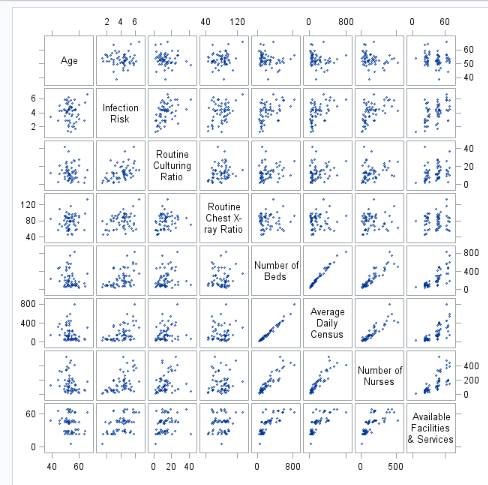
\includegraphics[scale=0.6]{14569224_800977350004906_642069745_n.png}
\caption{Scatterplot matrix. }
\end{figure}

\begin{figure}[H]
\centering
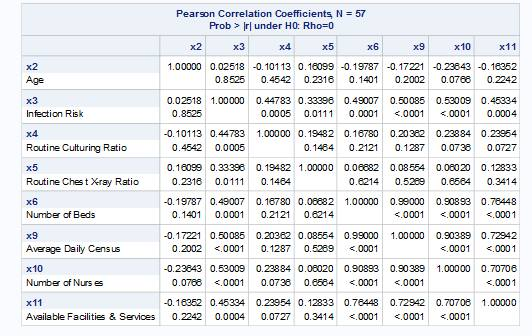
\includegraphics[scale=0.6]{14543358_800977370004904_386370053_n.png}
\caption{Correlation matrix of the X variables. }
\end{figure}

\end{document}
